\documentclass{article}

\usepackage{amsmath}
\usepackage{hyperref}
\usepackage{graphicx}
\usepackage{minted}
\usepackage[margin=1.5cm, includefoot, footskip=30pt]{geometry}


\title{Modelling Magic with Python: Ertai}
\author{Vince Knight}
\date{2021--04--16}

\begin{document}

\maketitle

\begin{abstract}
This paper introduces Ertai: a python library that allows for the mathematical
modelling of a popular Collectible Card Game (CCG): Magic the Gathering (MtG).

As well as describing the high level functionality of this library, a specific
use case will be given that allows for the calculation of a `Mana Curve' which
is of strategic interest to players of MtG.
\end{abstract}

\section{Introduction}

Magic the Gathering (MtG) is a Collectible Card Game (CCG) first released in
1993~\cite{mtg-wikipedia} and is arguably the first and most popular CCG\@.

The game has a number of strategic elements of gameplay:

\begin{enumerate}
    \item Card selection: from ones collection deciding which cards to use to
        form a \textit{deck}.
    \item In play strategy: during the play against an opponent, the large
        number of card combinations allow for many strategic possibilities.
    \item Card trading: by design cards have varying value and are often the
        subject of trades.
\end{enumerate}

The \mintinline{python}{ertai} library aims to allow for the simulation of
certain aspects of game play as applied to the first of these: how to select
cards in a specific way.

At its core MtG has a dynamic of casting spells (playing cards) which requires a
player to spend ``Mana''. This resource can be of various types, that correspond
to the colours of Magic in MtG: black, white, blue, red or green.

One of the things that can be done with \mintinline{python}{ertai} is an
arithmetic of Mana. For example, we can take a specific combination of Mana (1
Blue, 2 Red) away from a collection of 3 Blue, 2 Red and 1 Black Mana.

\begin{minted}{python}
>>> import ertai
>>> mana_cost = ertai.Mana("Blue", "Red", "Red")
>>> mana_pool = ertai.Mana("Blue", "Blue", "Blue", "Red", "Red", "Black")
>>> mana_cost <= mana_pool
True
>>> mana_pool - mana_cost
2 Blue Mana, 1 Black Mana

\end{minted}

As well as this, card objects can be created which allows for the modelling of
the card selection. For example, in Figure~\ref{fig:mana_curve} 
the proportion of the available resources used at each turn for 3 different
card selections is obtained through Monte Carlo simulation.

\begin{figure}[!htbp]
    \begin{center}
        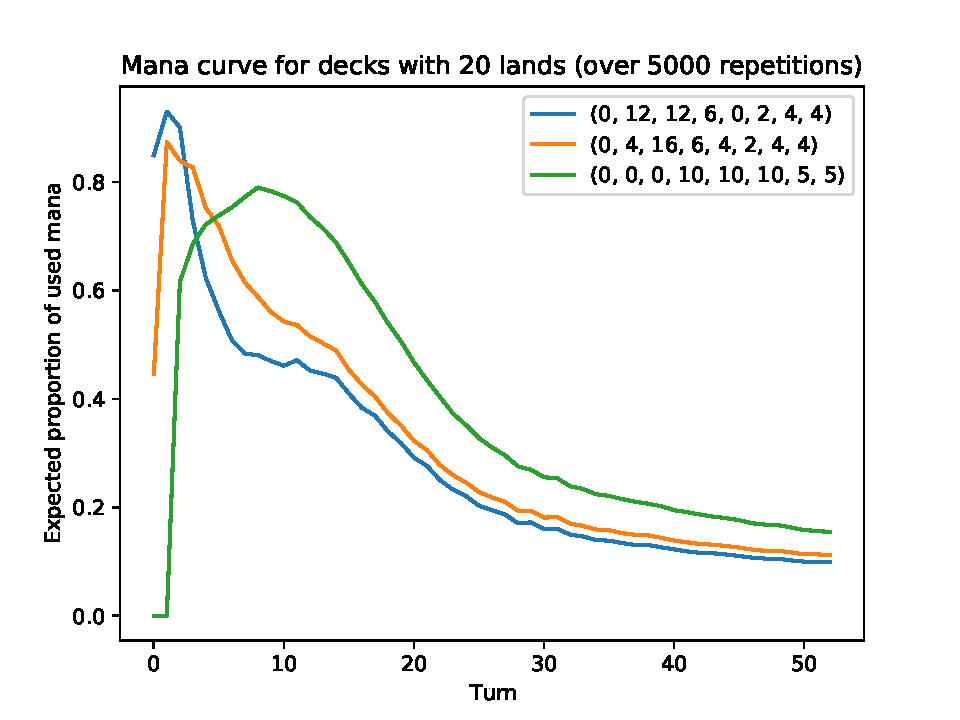
\includegraphics[width=.5\textwidth]{./img/mana_curve/main.pdf}
    \end{center}
    \caption{A mana curve: the proportion of available resources used at each
    turn for a given deck selection. The three selections represent number of
    cards of a given cost.}\label{fig:mana_curve}
\end{figure}

\section{Statement of need}

This type of analysis is not novel, for example~\cite{bjorke2017deckbuilding}
describes some academic work that aimed to optimise deck building (which is the
term used to describe card selection). This highlights that mathematical
modelling of MtG is of interest. Interestingly it is also studied in a social
science setting~\cite{vsvelch2020mediatization}.

In~\cite{bjorke2017deckbuilding} a number
of other libraries that can be used to simulate plays of the game are described,
for example: Magarena \url{https://magarena.github.io} which is an open source
library built in Java.

The \mintinline{python}{ertai} library is the first Python library (to the
authors knowledge) which allows it to be readily used in conjunction with other
scientific tools. Furthermore one particular goal of \mintinline{python}{ertai}
is to be specifically translatable to mathematical models of MtG.

\section{Conclusion}

This paper has given a description of \mintinline{python}{ertai}: a library with
a goal of allowing for the mathematical modelling of MtG.

The current capabilities of the library are limited but as it is written in
Python, the object oriented nature of the library can be used to make the
library extendable to other aspects of MtG. Every ability of a Magic card can be
added as a method on the \mintinline{python}{ertai.Card} class.

The library is written in a fully modular way, is well documented and is
automatically tested.

Furthermore, the library is already installable using standard python workflow:

\begin{minted}{bash}
    $ python -m pip install ertai
\end{minted}

The source code is available at \url{https://github.com/drvinceknight/ertai}.

\bibliographystyle{plain}
\bibliography{bibliography.bib}

\end{document}
